\documentclass[review]{elsarticle}
\usepackage{lineno,hyperref}
\modulolinenumbers[5]
\usepackage{dcolumn, graphics, graphicx, grffile, amsmath, amsthm, amssymb, color, colortbl}
\usepackage{subfig}
\usepackage{enumitem}
\usepackage{booktabs}
\usepackage{float}
\usepackage{geometry}
\geometry{verbose,tmargin=2.5cm,bmargin=2.5cm,lmargin=2.5cm,rmargin=2.5cm}
%\usepackage{authblk}
\usepackage[latin1]{inputenc}
\usepackage{tikz}
\usetikzlibrary{shapes,arrows}
\usepackage{verbatim}
\usepackage{setspace}
\usepackage{array}
\usepackage{multirow}
\usepackage{blkarray}
\usepackage{mathtools}
\usepackage{natbib}
% boldface lowercase letters for vectors
\newcommand{\xbf}{\ensuremath{\mathbf x}}

\journal{Spatial Statistics}
\bibliographystyle{model2-names.bst}\biboptions{authoryear}

\begin{document}
\begin{frontmatter}

\title{Grid-spacing and the quality of abundance maps for species that show spatial autocorrelation and zero-inflation}

%% Group authors per affiliation:
\author[1]{Olga Lyashevska}
\ead{olga@herenstraat.nl}

\author[2]{Dick J. Brus}
\ead{Dick.Brus@wur.nl}

\author[1]{Jaap van der Meer\corref{cor1}}
\ead{Jaap.van.der.Meer@nioz.nl}

\cortext[cor1]{Corresponding author}

\address[1]{Department of Marine Ecology\\
NIOZ Royal Netherlands Institute for Sea Research\\
P.O. Box 59 1790 AB Den Burg\\
Texel, The Netherlands}

\address[2]{Alterra, Wageningen University and Research Centre\\
P.O. Box 47, 6700AA\\
Wageningen, The Netherlands}

\begin{abstract}
The effect of grid-spacing on the quality of species abundance maps is explored for species that show zero-inflation and spatial autocorrelation.
Species abundance maps constructed through a generalised linear geostatistical modelling approach were subsampled by grid-sampling with 200, 400, 800, 1600, and 3200 m grid-spacing.
The model parameters at 1000 validation locations were predicted by simple kriging with an external drift, using silt, silt squared and altitude as external drift variables.
Two approaches were used for choosing kriging model parameters: fixed parent-model parameters and variable sample-specific parameters, giving a rough estimate of the sampling distribution.
A total of 100 grid-samples was obtained using the first approach and 4 grid-samples using the second approach.
Both approaches showed an increase in the Mean Squared Error with increasing spacing.
This increase, however,  was not smooth in the second approach but showed a steep rise at 3200 m when the number of sampling locations decreased from about 400 to about 200.
We therefore recommend to have at least 400 sampling locations.
\end{abstract}

\begin{keyword}
count data, generalized linear geostatistical modeling, autocorrelation, zero-inflation, grid-spacing
\end{keyword}

\end{frontmatter}

\linenumbers

\section{Introduction}

The relationship between species and their environment is generally described by species distribution models, also known as habitat suitability or environmental niche models \citep{guisan2005}. Such models are constructed using survey data available at a limited set of sampling locations and allow one to create predictive species distribution maps on the basis of environmental data which are usually available at a much larger set of locations \citep{guisan2000}. The number of sampling locations is known to affect the accuracy of the species distribution models and maps \citep{stockwell2002, wisz2008}.  Knowledge of the trade-off function between the number of sampling locations and the accuracy of the predictions is usually not obtained a priori  with the risk that the survey either does not provide the required accuracy or is unnecessarily costly \citep{caughlan2001,reynolds2011}.

Yet, the effect of sample size on the accuracy of species distribution models was evaluated by few \citep[see e.g.][]{stockwell2002,pearson2007,wisz2008,hanberry2012}. For example, \citet{stockwell2002} assessed sample size requirements for modelling bird species in Mexico by random sampling 1 to 100 locations. \citet{wisz2008} considered three sample sizes (10, 30, and 100 locations) to evaluate the quality of model predictions using data for 46 species obtained from natural history collections. Finally, \citet{hanberry2012} used sample sizes ranging from 30 to 2500 locations to model tree species in northeasten  Minnesota. All these studies consider presence--absence maps, but often, predictive species abundance maps in the form of numerical or biomass density are to be preferred,  because they are more informative than presence--absence maps \citep{vieira2012, cozzi2013}.  \citet{fortin1989} constructed such maps using sugar-maple tree density data gathered in  southwestern Qu\'{e}bec.  The authors evaluated the ability to predict spatial patterns using different sample sizes and designs. They considered two sample sizes of 50 and 64 points, both derived from a 200-point dataset.

Using real datasets only, as \citet{fortin1989} did, the possibilities of studying the effect of the type of sampling design and sample size are limited. This limitation was recognised in recent studies, such as those  by \citet{perner2004, rachowicz2006, bijleveld2012} and \citet{foster2014}. These studies follow an approach whereby first a spatial field resembling reality as much as possible, a peseudo-reality, is simulated, which is subsequently sampled using different sampling designs. The performance of sampling designs is then compared by confronting predictions with simulated values that serve as ground-truth.  \citet{zurell2010} call this the virtual ecologist approach.  Following this approach, \citet{bijleveld2012}, for example, used the results of an existing intertidal benthic monitoring programme to construct various spatial models with an exponential spatial autocorrelation function. With these models they simulated virtual populations with a Normal distribution and sampled these populations using different sampling designs. They provided a trade-off function between sampling distance and prediction error which was rather flat for those virtual species that hardly showed spatial autocorrelation, but much steeper for species with strong spatial autocorrelation. The authors assumed normality of the data which was clearly violated by the empirical data if only because of the many zero observations.

The assumption of normality is a common practice, but when we are dealing with species abundance (count) data, even the more obvious Poisson distribution is rarely applicable. Ecological count data have two properties that ask for a specific treatment, other than relying on the classical assumption of independent and normally distributed data. These properties are zero-inflation \citep{martin2005, clarke1988, lewis2011} and spatial autocorrelation, i.e. nearby observations are more similar than observations far apart, even when environmental conditions do not differ. Hitherto most studies have dealt with these two properties, but only one at a time \citep{tyre2003, bijleveld2012}.

For example, the first property was accounted by \citet{tyre2003} who considered the zero-inflated negative binomial model, but ignored autocorrelation. Ignoring spatial autocorrelation in simulation studies on how sampling designs affect the accuracy of estimates of population- or model parameters or the accuracy of spatial predictions, may lead to biased estimates of this accuracy \citep{legendre2002}.

Contrary to \citet{tyre2003}, the \citeauthor{bijleveld2012} study took account of the autocorrelation by using a stochastic model that included spatial autocorrelation of the error. But, as we mentioned earlier, they simulated normally distributed data. Clearly, there is a need to integrate both properties in a single study and to examine how zero-inflation and autocorrelation may affect recommendations concerning the optimal sampling design, sample size, and distance between samples.

Only few studies simultaneously address zero-inflation and autocorrelation for species abundances \citep[see e.g.][]{recta2012, boyd2015}, but none of them address the question of optimal sampling design.  We fill this gap by following a paper by \citet{lyashevska2015a} in simulating fields with zero-inflated, spatially autocorrelated count data, and sampling the fields repeatedly with different sampling designs. More specifically, we will sample the fields by grid-sampling with a varying spacing. The objective of this paper is to quantify the trade-off between the grid-spacing and the accuracy of predictions of species-abundance model parameters on a fine grid for mapping, for species that show zero-inflation and spatial autocorrelation. Most species will show these two properties.

\section{Materials and methods} \label{sec:methods}

%We provide a brief description of the statistical methodology of modelling zero-inflated, auto-correlated species abundance data. For more details we refer to the companion paper \citep{lyashevska2015}.

\subsection{Data}

Data used in this paper were zero-inflated (66\% are zeros) and autocorrelated counts of a benthic species \textit{Macoma balthica} (Fig.~\ref{fig:AbundanceRaw}) that were collected in the yearly Synoptic Intertidal Benthic Surveys (SIBES) monitoring programme conducted in the Dutch Wadden Sea \citep{bijleveld2012, compton2013}. The study area, bordered by the barrier islands on the north and by the mainland coast on the south, is formed by intertidal and subtidal mudflats and gullies. The monitoring network consists of 3451 permanent locations on intertidal mudflats at the nodes of a 500 m grid. The square grid is supplemented by 578 locations. These locations were selected by first selecting 578 out of the 3451 grid-points by simple random sampling without replacement. Then at each selected grid-point one point was selected at a uniformly distributed distance between 0 and 250 m distance from the grid-point, in a direction randomly chosen from the four directions defined by the grid-lines \citep{bijleveld2012}.

The most important determinants of habitat structure used for mapping the abundance were sediment texture characteristic, more specifically the mass fraction of silt, and altitude (Amsterdam Ordnance Datum, Rijkswaterstaat \footnote{www.rijkswaterstaat.nl}). To be used as a predictor in mapping, the covariate must be known everywhere in the study area. Therefore the mass fraction of silt was interpolated by inverse distance weighting in ArcGIS 10.0.

\subsection{Overview of evaluation method}
The starting point of the our procedure for evaluating the sampling designs is a model for the spatial distribution of the zero-inflated and autocorrelated count data. This spatial distribution is modelled through a spatial zero-inflated Poisson mixture model(ZIP)\citep{lambert1992, agarwal2002}:
\begin{equation}
    P(Y_i=y)=
\begin{cases}
\pi_i+(1-\pi_i)\text{exp}(-\mu_i) & y=0 \\
(1-\pi_i)\frac{\text{exp}(-\mu_i)\mu_i^{y}}{y!}& y=1,2,3,\ldots
\end{cases}
\end{equation}
where $Y_i$ is the count at location $i$, $\pi_i$ the probability of a Bernoulli zero at location $i$, and $1-\pi_i$ is the probability of a Poisson count, either zero or non-zero. The intensity (mean number of individuals) of the Poisson process at location $i$ is $\mu_i$. The first part of the model is the overall probability of zero \citep{hilbe2007}.

The parameters $\pi_i$ and $\mu_i$ at location $i$ are random variables modelled by the following submodels:
\begin{eqnarray} \label{eq:glsm}
\text{logit}(\pi_{i})=\text{log}(\frac{\pi_{i}}{1-\pi_{i}})=\xbf_{\mathrm{B},i}^{T}\boldsymbol{\beta}_{\rm{B}} + \eta_{\mathrm{B},i} \nonumber \\
\text{log}(\mu_i)=\xbf_{\mathrm{P},i}^{T}\boldsymbol{\beta}_{\rm{P}} + \eta_{\mathrm{P},i}
\end{eqnarray}
with $\xbf_{\mathrm{B},i}$ and $\xbf_{\mathrm{P},i}$ vectors with covariates at location $i$, $\boldsymbol{\beta}_{\mathrm{B}}$ and $\boldsymbol{\beta}_{\mathrm{P}}$ vectors with regression coefficients, and $\eta_{\mathrm{B},i}$, $\eta_{\mathrm{P},i}$ residuals of the spatial trend. Note that the model parameters can be modelled by different sets of covariates.

The residuals $\eta_{\mathrm{B},i}$, $\eta_{\mathrm{P},i}$ at any location $i$ are random variables. The probability distribution of the residuals at all locations in the study area was modelled as
\begin{eqnarray}
\left[
\begin{array}{c}
\boldsymbol{\eta}_{\mathrm{B}} \\
\boldsymbol{\eta}_{\mathrm{P}} \\
\end{array}
\right]&\sim& \mathcal{N}\left(
\left[
\begin{array}{c}
\mathbf{0} \\
\mathbf{0} \\
\end{array}
\right],
\left[
\begin{array}{cc}
\mathbf{C}_{\mathrm{B}} & \mathbf{0} \\
\mathbf{0} & \mathbf{C}_{\mathrm{P}} \\
\end{array}
\right]
\right)
\end{eqnarray}
with $\mathbf{C}_{\mathrm{B}}$ and $\mathbf{C}_{\mathrm{P}}$ covariance matrices. So note that we assumed that the Bernoulli and Poisson residuals were independent. For both random residuals we further assumed isotropy, so that the covariance of the residuals at any two locations was modelled as a function of the distance $h$ between the two locations. For instance, for the Bernoulli residuals, the covariance was modelled as
\begin{equation}
    C_{\mathrm{B}}(h)=\sigma_{\mathrm{B}}^{2}\rho_{\mathrm{B}}(h; \phi_{\mathrm{B}})+\tau_{\mathrm{B}}^{2} \label{Ch}
\end{equation}
with $\sigma_{\mathrm{B}}^{2}$ the partial sill, $\phi_{\mathrm{B}}$ the range (distance parameter), $\tau_{\mathrm{B}}^{2}$ the nugget, and $\rho_{\mathrm{B}}$ the correlation function, for instance exponential or spherical \citep{webster2007}.

The two submodels in ~\ref{eq:glsm} are generalised linear mixed models, as they are the sum of a linear combination of covariates describing a spatial trend (fixed effect) and a spatially autocorrelated residual (random effect). \citet{diggle2007} names this type of models as generalised linear \textit{geostatistical} models.

Following \citet{diggle2007}, hereafter the sum of the trend and residual, representing the transformed model parameter, is referred to as the signal $S$, for instance $S_{\mathrm{B},i}= \mathbf{x}_{\mathrm{B},i}^{T}\boldsymbol{\beta}_{\rm{B}} + \eta_{\mathrm{B},i}$. For convenience, all the parameters in one model, including the type of correlation function, are collected in  a vector: $\boldsymbol{\theta}_{\mathrm{B}}=(\boldsymbol{\beta}_{\mathrm{B}}, \phi_{\mathrm{B}}, \tau_{\mathrm{B}}^2, \sigma_{\mathrm{B}}^2, \rho_{\mathrm{B}})$ and $\boldsymbol{\theta}_{\mathrm{P}}=(\boldsymbol{\beta}_{\mathrm{P}}, \phi_{\mathrm{P}}, \tau_{\mathrm{P}}^2, \sigma_{\mathrm{P}}^2, \rho_{\mathrm{P}})$. To avoid confusion the model parameters $\boldsymbol{\theta}_{\mathrm{B}}$ and $\boldsymbol{\theta}_{\mathrm{P}}$ are referred to as hyperparameters; with model parameters we mean the parameters $\pi$ and $\mu$.

The aim of the sampling strategy to be evaluated is to map the prevalence parameter $\pi$ of the Bernoulli distribution and the intensity parameter $\mu$ of the Poisson distribution. So note that the aim is not to predict the species abundance counts, but the \emph{expected} counts, conditional on covariates that define a spatial trend and the observed counts at the sample to be evaluated. We believe that predicting the counts themselves is not feasible in our situation, and besides not of practical relevance.

Broadly speaking, our evaluation procedure is as follows. The SIBES data are used to calibrate a ZIP model. Several steps are involved in calibration. First, a ZIP model is fitted by maximum likelihood assuming that both residuals $\eta_{\mathrm{B},i}$ and $\eta_{\mathrm{P},i}$ are spatially independent. The fitted model parameters are then used to classify a zero count either as a Bernoulli or a Poisson zero, and to construct two datasets: the Bernoulli dataset with zeros (absent) and ones (present), and the Poisson subset, containing the SIBES locations with a one in the Bernoulli dataset, with counts. In the next step these two data sets are used to fit the two submodels for the parameters $\pi_i$ and $\mu_i$, but now accounting for spatial autocorrelation. This is done by simulating a large sample of signals $S_{\mathrm{B}}$ and $S_{\mathrm{P}}$ at the SIBES locations by Markov chain Monte Carlo (MCMC) using initial estimates of the hyperparameters, followed by Monte Carlo Maximum Likelihood (MCML) estimation of the hyperparameters.

The fitted hyperparameters are then used to predict the Bernoulli signal ($S_{\mathrm{B}}$) and Poisson signal ($S_{\mathrm{P}}$) at the nodes of a very fine square grid with a spacing of 100 m covering the study area. This prediction grid is extended with 1000 randomly selected validation locations in between the grid-points. The prediction method is simple kriging with an external drift, using silt, the squared values of silt, and altitude as external drift variables (predictors).

In the next step the predicted signals at the grid-nodes and validation points are used to simulate fields with count data. One field with statistics closest to those of the SIBES data is selected, and repeatedly sampled by grid-sampling. A range of grid-spacings is applied. Each selected grid is used to predict the model parameters $\pi_i$ and $\mu_i$ at the validation locations. By comparing these predictions with the true model parameters at the validation points the quality of the predictions is assessed. More details on all steps but the first two (calibration of ZIP model and prediction of signals) are given below. For details on the first two steps we refer to \citet{lyashevska2015a}.

\begin{enumerate}
\item
After prediction of the signal $S_{\mathrm{B}}$ at the nodes of the 100 m grid, 100 fields (square grids with spacing of 100 m) with spatially unstructured noise (white noise) are simulated from a Normal distribution with a variance equal to $\hat{\tau}^2_{\mathrm{B}}$. The predicted signal ($S_{\mathrm{B}}$) is added to the simulated fields with white noise. The resulting fields are backtransformed by second-order Taylor expansion to give 100 simulated fields of the prevalence parameter $\pi$ of the Bernoulli distribution. The same procedure is followed for the $S_{\mathrm{P}}$ to give 100 simulated fields of the intensity parameter $\mu$ of the Poisson distribution.

\item
Each simulated field of $\pi$ is used to simulate one field with presence/absence indicators, giving 100 fields with indicators. Besides, each simulated field of $\mu$ is used to simulate one field with Poisson counts, giving 100 fields with counts. These two sets of 100 fields are multiplied pair-by-pair, to give 100 fields with zero-inflated counts.

\item
From the 100 fields with zero-inflated counts, one field is selected with summary statistics closest to these summary statistics of the SIBES data. We used as summary statistics the fraction of zeroes, the mean of the Poisson counts, and the variance of the Poisson counts. This leads to three difference values per field. These differences values were standardized by dividing through their standard deviation. The weighted sum of the standardized differences was used as a selection criterion, with weights equal to 0.5 (for fraction of zeroes), 0.25 and 0.25. Apart from the field with zero-inflated counts, the two underlying fields with simulated prevalence parameter values $\pi$ and simulated intensity parameter values $\mu$ are selected, as these are needed in the validation (remind that the aim was to predict the model parameters $\pi$ and $\mu$). Fig.~\ref{fig:rawfield} shows a map of the product of $\pi$ and $\mu$, representing the unconditional intensity (unconditional expected count), and a map of the SIBES count data. There is a clear resemblance between the two maps.

\begin{figure}[htbp]
\subfloat[]{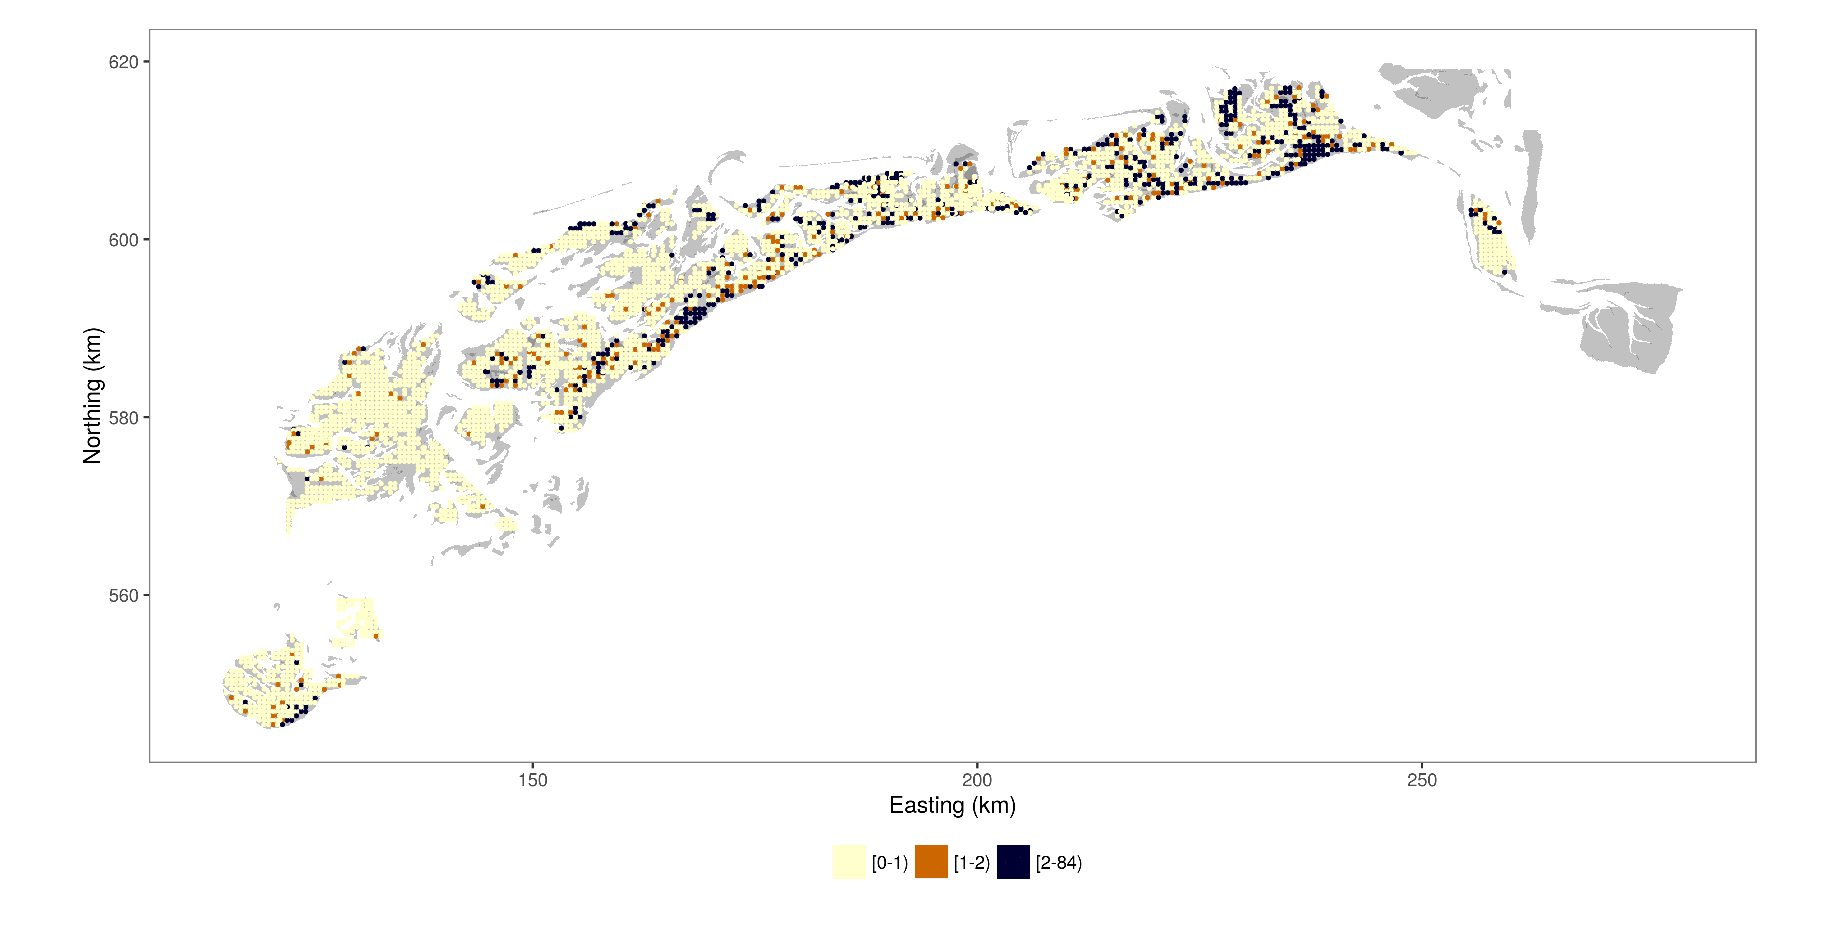
\includegraphics[width=0.9\linewidth]{AbundanceRaw} \label{fig:AbundanceRaw} }\quad
\subfloat[]{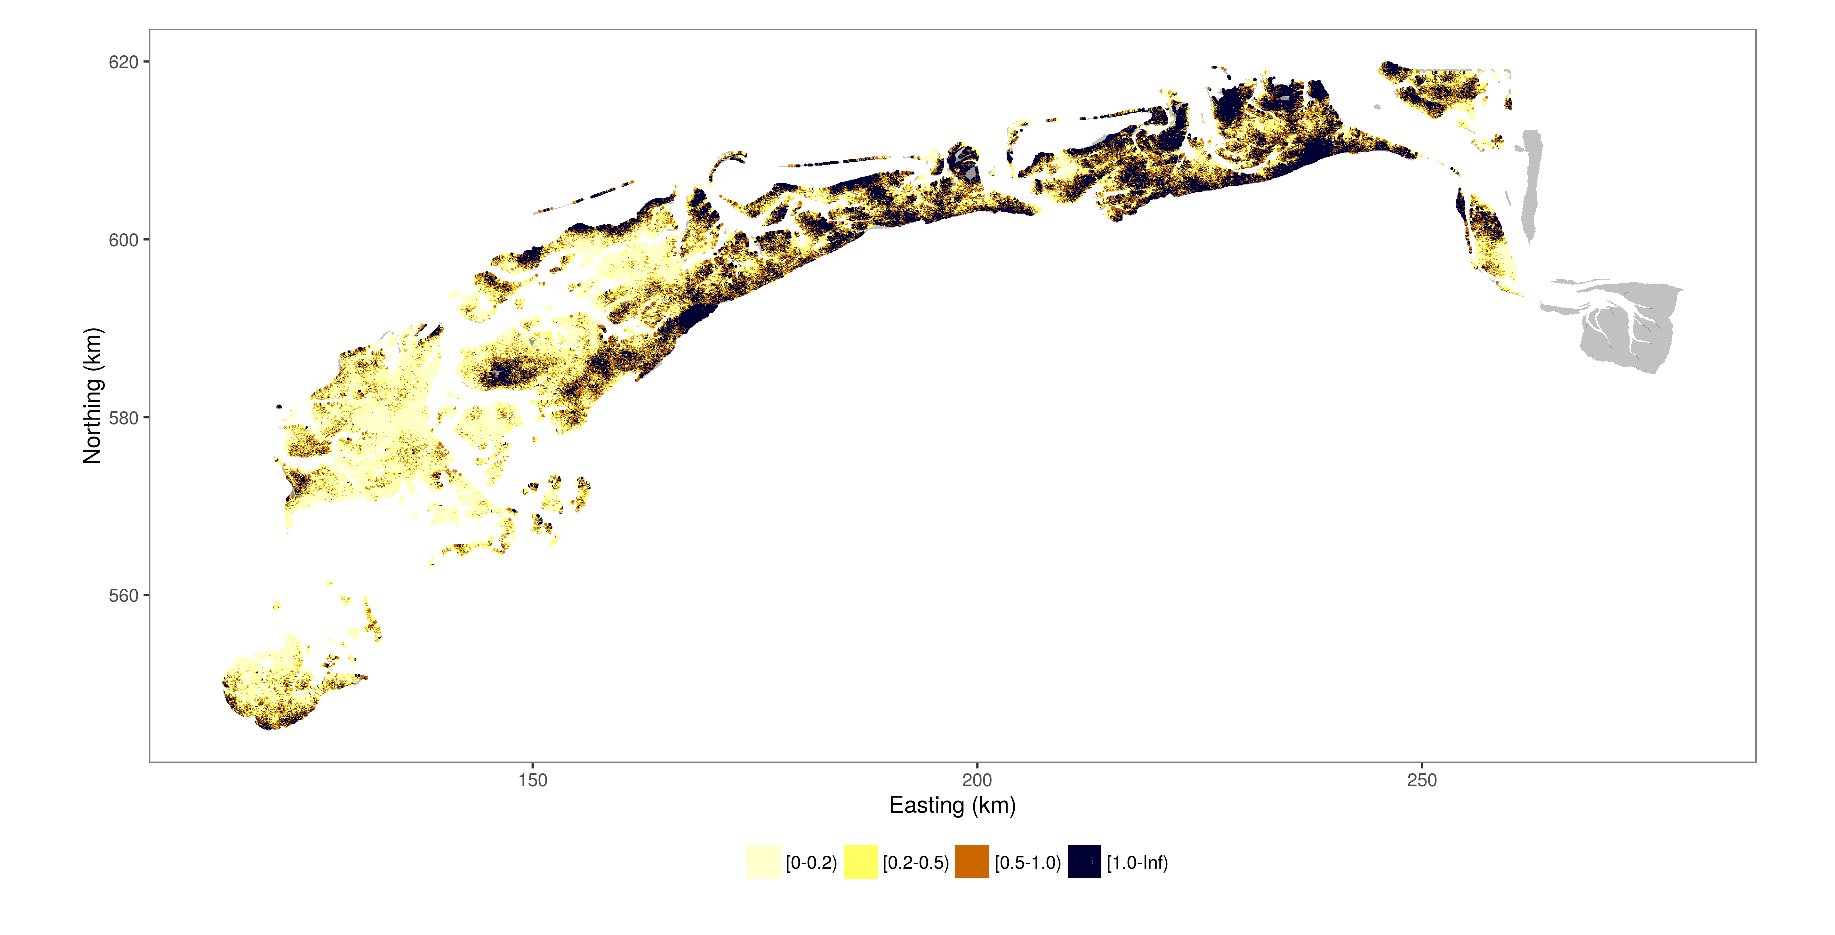
\includegraphics[width=0.9\linewidth]{pred.pimu.eps} \label{fig:field38} }
\caption{Empirical species abundance map of \textit{Macoma balthica} \protect\subref{fig:AbundanceRaw} and unconditional intensity map \protect\subref{fig:field38} predicted to the nodes of 100 m grid by simple kriging with an external drift. From \citet{lyashevska2015a}.}
\label{fig:rawfield}
\end{figure}

\item
The selected field with zero-inflated counts is sampled on a grid with a spacing of 200, 400, 800, 1600, and 3200 m. For each grid-spacing 100 samples are randomly selected. The corresponding number of grid-points was on average 28505, 7130, 1783, 446, and 110, respectively. An overlay is made of the selected grids and the selected field with simulated zero-inflated counts to obtain the `pseudo-observations' of counts that will be used in prediction of the prevalence parameter $\pi$ and the intensity parameter $\mu$ at the validation locations.

\item
The model parameters $\pi$ and $\mu$ at the 1000 validation locations are predicted by the same method as used in simulating our pseudo-reality, being simple kriging with an external drift, using silt, silt-squared and altitude as external drift variables. Ideally, for each grid-sample the hyperparameters are estimated from the `pseudo-observations' of zero-inflated counts at the grid-points with Markov chain Monte Carlo maximum likelihood (MCML). However, this is not feasible due to the computing time involved. Therefore, in predicting from the selected grid-points to the validation points we used the hyperparameters that were also used to simulate all 100 fields. These hyperparameters (referred to hereafter as the parent-hyperparameters) were estimated by MCML from the SIBES data. In practice these hyperparameters are unknown, so that by using the unknown parent-hyperparameters we ignore the contribution of uncertainty about the hyperparameters to the uncertainty about the predictions.

To obtain a rough idea about this contribution, per grid-spacing four grid-samples are selected that are used to estimate the hyperparameters. As a consequence the hyperparameters are not fixed but vary between the four samples of a given grid-spacing. The hyperparameters are not estimated from the pseudo-observations of zero-inflated counts at the selected grid-points, but from the Bernoulli and Poisson signals at these points. In doing so we avoid the time-demanding MCML estimation. By using the simulated signals as observations the hyperparameters can be estimated by Residual Maximum Likelihood (REML). We are aware that this estimation procedure does not reflect practice either, and that the contribution of uncertainty about the hyperparameters will be underestimated, but we see it as a first attempt within reasonable computing time.
\end{enumerate}

\subsection{Quality measures}
The quality of the predicted prevalence parameters was quantified by the Mean Squared Error (MSE); for instance for the prevalence parameter $\pi$ this MSE equals :
\begin{equation}
    \text{MSE}(\pi)=\frac{1}{n}\sum_{i=1}^{n} \left\{\hat{\pi_{i}} - \pi_{i} \right\}^{2}
\label{eq:mse}
\end{equation}
with $n$ the number of validation points ($n=1000$), $\hat{\pi_{i}}$ the predicted prevalence parameter at location $i$ and $\pi_{i}$ the `pseudo-observed' intensity parameter. For intensity parameter $\mu$ MSE is computed from the subset of validation points with a simulated 1 (species present). This subset contains 211 points. MSE was also calculated for the product of $\pi$ and $\mu$, representing unconditional intensity (intensity not conditioned on presence). For this product again all 1000 validation are used.

For each grid-spacing we have 100 grid-samples. All 100 grid-samples are used in prediction with the fixed parent-hyperparameters $\boldsymbol{\theta}_{\mathrm{B}}$ and $\boldsymbol{\theta}_{\mathrm{P}}$ (no sample-specific estimation), leading to 100 estimates of MSE$(\pi)$, MSE$(\mu)$ and MSE$(\pi \cdot \mu)$. The distribution of these 100 estimates is an estimate of the sampling distribution of the estimated mean quality of model-based predictions of the model parameters $\pi$ and $\mu$. Only four grid-samples are used in prediction with variable sample-specific estimates of the hyperparameters $\boldsymbol{\theta}_{\mathrm{B}}$ and $\boldsymbol{\theta}_{\mathrm{P}}$, so these four estimates give a very rough estimate of the sampling distribution only.

\section{Results} \label{sec:results}

\subsection{Prevalence}
The mean of MSE of the predicted species prevalence parameter $\pi$ increased with increasing grid-spacing (Fig.~\ref{fig:mse.pi}).
Using the fixed parent-hyperparameters the increase was from a value close to 0 at 200 m to 0.001 at 3200 m. Except for the largest spacing of 3200 m, the variance of MSE between the 100 grid samples was small.

The mean of the four MSE values using hyperparameters estimated from the grid-samples, was for all spacings larger than the mean of MSE using the fixed parent-hyperparameters, especially for the largest spacing. This shows that the contribution of uncertainty about the hyperparameters to the uncertainty about the predictions was substantial. Remarkable is the strong increase of the mean MSE beyond a spacing of 1600 m.

\begin{figure}[htbp]
\subfloat[]{\includegraphics[width=.49\linewidth]{mse.pi} \label{fig:mse.pi}}\quad
\subfloat[]{\includegraphics[width=.49\linewidth]{mse.mu1} \label{fig:mse.mu}}\quad
\subfloat[]{\includegraphics[width=.49\linewidth]{mse.pimu}\label{fig:mse.pimu}}\\
\caption{The MSE for predicted prevalence ($\pi$) \protect\subref{fig:mse.pi}, predicted intensity ($\mu$) \protect\subref{fig:mse.mu} and predicted unconditional intensity ($\pi \cdot \mu$) \protect\subref{fig:mse.pimu} as a function of grid-spacing for 200, 400, 800, 1600, and 3200 m. Predictions were obtained by simple kriging with an external drift with fixed parent-hyperparameters (blue) and hyperparameters estimated from a sample (red). The first grid-spacing (200 m) with estimated hyperparameters could not be estimated due to memory constraints.}
\label{fig:mse}
\end{figure}

\subsection{Intensity}
Similar to the prevalence parameter $\pi$, the  mean of MSE of the predicted intensity parameter $\mu$ increased with increasing grid-spacing (Fig.~\ref{fig:mse.mu}). Using fixed parent-hyperparameters the increase was from 0.26 at 200 m to 12.25 at 3200 m (Fig.~\ref{fig:mse.mu}). Using hyperparameters estimated from the grid-samples, the mean of MSE increased even more, from 2.41 for 400 m (compared with 0.7 at 400 m for fixed hyperparameters) to 13.82 at 3200 m.  In contrast to the prevalence parameter $\pi$ the mean MSE already started to increase strongly at spacings beyond 400 m.

The  graph of the MSE for the product of $\pi$ and $\mu$ is very similar to the graph for the prevalence parameter $\pi$. For the first four spacings the increase of the mean MSE was very modest, but beyond a spacing of 1600 m, the increase was much stronger (Fig.~\ref{fig:mse.pimu}).

DICK: IK KAN DIE SMOOTHING NIET ZIEN OP DE KAARTJES, DAARVOOR ZIJN DE KLASSEN TE BREED. IM DENK DAT JE DEZE SMOOTHING DUS ANDERS MOET PRESENTEREN, BIJV. IN EEN TABEL OF GRAFIEK (BOXPLOTS VAN PREDICTIES). Visual comparison of the maps of unconditional intensity predicted by simple kriging with sample estimated hyperparameters reveals progressive smoothing of predictions as grid-spacing increases (Fig.~\ref{fig:pr.pimu.reml}). The predicted unconditional intensity varied between 0.02 and 14.9 (mean 0.85, sd 1.31) for 400 m grid (Fig.~\ref{fig:pr.pimu.remla}) and between 0.07 and 18.19 (mean 0.92, sd 0.96) for 3200 m grid (Fig.~\ref{fig:pr.pimu.remld}).

\begin{figure}[htbp]
    \subfloat[]{\includegraphics[width=0.49\linewidth]{pr.pimu400}\label{fig:pr.pimu.remla}}\quad
    \subfloat[]{\includegraphics[width=.49\linewidth]{pr.pimu800}\label{fig:pr.pimu.remlb}}\\
    \subfloat[]{\includegraphics[width=0.49\linewidth]{pr.pimu1600}\label{fig:pr.pimu.remlc}}\quad
    \subfloat[]{\includegraphics[width=0.49\linewidth]{pr.pimu3200}\label{fig:pr.pimu.remld}}\\
\caption{Unconditional intensity predicted at 1000 validation points by simple kriging with an external drift with variable sample-specific model parameters from 400 \protect\subref{fig:pr.pimu.remla}, 800 \protect\subref{fig:pr.pimu.remlb}, 1600 \protect\subref{fig:pr.pimu.remlc}, and 3200 \protect\subref{fig:pr.pimu.remld} m grid. An average of 4 grid-samples.}
\label{fig:pr.pimu.reml}
\end{figure}

\section{Discussion and conclusions}\label{sec:discussion}
The objective of this paper was to quantify the effect of the grid-spacing on the quality of spatial predictions of abundance of species that show zero-inflation and spatial autocorrelation. We proposed an approach in which multiple fields of the prevalance parameter $\pi$ and the intensity parameter $\mu$ of a zero-inflated Poisson mixture model are simulated by generalized linear geostatistical models. These fields were used to simulate pseudo-realities of zero-inflated autocorrelated counts. One pseudo-reality was then selected with summary statistics that were close to summary-statistics of the available data. This pseudo-reality was then sampled by the sampling design under study, in this study grid-sampling at various grid-spacings. A selected sample was used to predict at a fixed set of validation locations and to compute the MSE of the predictions of $\pi$ and $\mu$. By repeating the selection of samples and the prediction at the validation points, an estimate of the sampling distribution of MSE is obtained.

To construct the graph with the estimated sampling distribution of MSE against grid-spacing the hyperparameters that were used to simulate the pseudo-reality were also used in spatial prediction at the validation points. As a consequence, this graph shows the effect of the grid-spacing \emph{given the model}. This is common practice in designing spatial samples for mapping by kriging. \citet{mcbratney1981} optimized  the spacing of grids using as an evaluation criterion the maximum kriging variance as obtained with ordinary kriging. Uncertainty about the variogram used in ordinary kriging is not accounted for. 
\citet{vangroenigen1999} optimized the spatial coordinates of a given number of sampling locations for ordinary kriging, also assuming that the variogram is known. \citet{brus2007} did the same for kriging with an external drift (KED). This study resembles the study described here, apart from that a linear mixed model is used instead of a generalized linear mixed model. The variance as computed with KED does account for uncertainty about the trend coefficients, but does not account for uncertainty about the variogram parameters, so also in this study the contribution of uncertainty about the variogram parameters is ignored.

Alternatively, in order to account for the uncertainty about the hyperparameters in estimating the MSE, the hyperparameters that are used in prediction are estimated from the samples. By repeatedly selecting samples with a given sampling design, estimating the hyperparameters, and predicting at the validation points, a sampling distribution of the MSE is obtained with a mean that will be larger than that of the sampling distribution of MSE obtained with the fixed parent-hyperparameters. The difference in the sampling distributions of MSE reflects the contribution of the uncertainty about the hyperparameters to uncertainty about the predictions due to sampling errors in the estimated hyperparameters.

This procedure for evaluating sampling designs is relatively simple and versatile. However, the applicability of this approach in our case study was hampered by the computing time involved in estimating the hyperparameters from a sample. In the proposed model for the zero-inflated counts spatial dependency is introduced at the level of the model parameters $\pi$ and $\mu$, which cannot be directly observed. Besides, both model parameters are non-linearly related to environmental covariates. The parameters of such model can be estimated by Monte Carlo Maximum Likelihood (MCML), which involves repeated simulation of long Markov chains, which is time consuming. As an approximation we estimated the hyperparameters by REML from the unobservable model parameters $\pi$ and $\mu$ at the selected sampling locations. Most likely this approximation underestimates the contribution of the uncertainty about the hyperparameters to the uncertainty about the predictions, but it is a first attempt within reasonable computing time. To improve the quality of the estimated MSEs at various grid-spacings a more efficient procedure for estimating the hyperparameters is needed. We welcome research into estimation of the hyperparameters of a ZIP mixture model by integrated nested Laplacian approximation, as proposed by \citet{rue2009}.

For the time being we must base our decisions on the graphs as presented in Figs~\ref{fig:mse.pi}, ~\ref{fig:mse.mu} and ~\ref{fig:mse.pimu}. The graphs of the prevalence parameter $\pi$ and of the unconditional intensity $\pi \cdot \mu$ show that beyond a spacing of 1600 m the mean of MSE starts increasing at a much faster rate. This is especially true for the MSEs obtained with hyperparameters estimated from the samples. Based on these findings the 1600 m grid which consists of 446 locations for our study area of 2400 km$^{2}$ seems to be a good compromise between sampling costs and prediction accuracy. The increase in accuracy of the 800 m grid does not seem to outweigh the fourfold increase in number of sampling units taken. But of course the optimal spacing can only be determined when sampling costs and accuracy are defined in a common unit.

\section*{Acknowledgements}

This study was part of the Wadden Long-Term Ecosystem Research (WaLTER) project, that is financially supported by the Waddenfonds, and the provinces of Frysl\^{a}n and Noord Holland. We thank the SIBES core-team, numerous volunteers, and the crew of the RV Navicula.
In 2010 the SIBES-monitoring was carried out with financial support from NAM, NWO-ALW (ZKO programme) and Royal NIOZ.

\section*{References}
\bibliography{ref}
\end{document}

The alternative would be to draw multiple vectors with model-parameters from the multivariate uncertainty distribution of the model-parameters, and use these one-by-one in prediction. This increase in MSE then reflects model-uncertainty about the model-parameters. 
